\documentclass[12pt,a5paper,titlepage, main = russian]{article}
\usepackage[T1,T2A]{fontenc}
\usepackage[utf8]{inputenc}
\usepackage[warn]{mathtext}
\usepackage{textcomp}
\usepackage[russian]{babel}
\usepackage{extsizes}
\usepackage[left = 1 cm, right = 1 cm, top = 1.5 cm, bottom = 1.5 cm]{geometry}
\usepackage [pagestyles, raggedright]{titlesec}
\usepackage{graphicx}
\usepackage{ragged2e}
\usepackage{amsmath}
\usepackage{pgfplots}
\pagestyle{empty}
\usepackage{tikz}
\usetikzlibrary{patterns}

\usepackage{wrapfig}

\usepackage{siunitx} % Required for alignment
\usepackage{multirow}
\usepackage{rotating}
\usepackage{float}
\usepackage{booktabs}

\usepackage{amsmath,amsfonts,amssymb,amsthm,mathtools} % AMS
\usepackage{icomma}
\usepackage[russian]{babel}
\usepackage[T2A]{fontenc}
\usepackage[utf8]{inputenc}
\usepackage{mathtext}
\usepackage{amsfonts}
\usepackage{ amssymb }
\usepackage{amsmath}
\usepackage{graphics}
\usepackage{graphicx}
\usepackage{wrapfig}
\usepackage{geometry}
\usepackage{float}

\usepackage{wrapfig}
\usepackage{graphicx}
\usepackage{mathtext}
\usepackage{amsmath}
\usepackage{siunitx} % Required for alignment
\usepackage{subfigure}
\usepackage{multirow}
\usepackage{rotating}
\usepackage{afterpage}
\usepackage[T1,T2A]{fontenc}
\usepackage[russian]{babel}
\usepackage{caption}
\usepackage[arrowdel]{physics}
\usepackage{booktabs}
\usepackage{float}


\begin{document}

\begin{titlepage}
\begin{center}
    \small{Министерство науки и высшего образования Российской Федерации}\\
    ФЕДЕРАЛЬНОЕ ГОСУДАРСТВЕННОЕ АВТОНОМНОЕ ОБРАЗОВАТЕЛЬНОЕ УЧРЕЖДЕНИЕ ВЫСШЕГО ОБРАЗОВАНИЯ "МОСКОВСКИЙ ФИЗИКО-ТЕХНИЧЕСКИЙ ИНСТИТУТ (НАЦИОНАЛЬНЫЙ ИССЛЕДОВАТЕЛЬСКИЙ УНИВЕРСИТЕТ)"\\
    (МФТИ, Физтех)
\end{center}
\vspace{2.5cm}
{\huge
    \begin{center}
        {\bf Отчёт о выполнении лабораторной работы}\\
        Эффект Зеемана
    \end{center}
}
\vspace{1.5cm}
\begin{flushright}
    {\large Авторы:\\  
Кулиш Павел \\
        \vspace{0.2cm}
        
        Б03-303}
\end{flushright}
\vspace{0.3cm}
\begin{center}
        Москва, \\
        Долгопрудный, 2026 г
\end{center}

\end{titlepage}


\tableofcontents
\newpage

\section{Цель работы}
Цель работы – изучение характеристик интерферометра Фабри–Перо (ИФП) и исследование эффекта Зеемана на примере расщепления линии ртути (\(\lambda = 579\) нм) в магнитном поле. 

\section{Теоретическая справка}
\subsection{Эффект Зеемана}
Эффект Зеемана заключается в расщеплении спектральных линий при помещении источника в магнитное поле. Различают простой (нормальный) и сложный (аномальный) эффект.

\subsubsection{Классическая интерпретация}
В классической модели Лоренца электрон в атоме рассматривается как гармонический осциллятор. В магнитном поле на электрон действует сила Лоренца, что приводит к расщеплению частоты на три компоненты:
\[
\omega = \omega_0 \pm \Delta\omega,\quad \Delta\omega = \frac{eH}{2mc},
\]
где \(\omega_0\) – частота без поля, \(H\) – напряжённость магнитного поля (в гауссах). 
В шкале волновых чисел:
\[
\Delta\nu = \frac{e}{4\pi m c} H\ (\text{см}^{-1}).
\]
При наблюдении поперёк поля видны все три компоненты (линейно поляризованные: \(\pi\) – не смещённая, \(\sigma\) – смещённые). Вдоль поля видны только две \(\sigma\)-компоненты с круговой поляризацией.
\subsubsection{Квантово-механическая интерпретация}
Для объяснения аномального эффекта Зеемана Уленбек и Гаудсмит ввели понятие спина электрона. 
Магнитный момент электрона складывается из орбитального и спинового:
\[
\mu_{\text{орб}} = \frac{e}{2mc}\hbar,\quad \mu_{\text{спин}} = \frac{e}{mc}\hbar.
\]
Полный магнитный момент определяется фактором Ланде \(g\).

В магнитном поле уровень энергии расщепляется на подуровни:
\[
E = E_0 + \mu_B H M g,
\]
где \(\mu_B = e\hbar/(2mc)\) – магнетон Бора, \(M\) – магнитное квантовое число, \(g\) – фактор Ланде:
\[
g = 1 + \frac{J(J+1) + S(S+1) - L(L+1)}{2J(J+1)}.
\]
Правила отбора для дипольного излучения: \(\Delta M = 0, \pm 1\). 
Компонента \(\Delta M = 0\) (\(\pi\)) линейно поляризована вдоль поля, \(\Delta M = \pm 1\) (\(\sigma^{\pm}\)) – циркулярно поляризованы при наблюдении вдоль поля и линейно (перпендикулярно полю) при поперечном наблюдении.

Величина расщепления компонент в волновых числах:
\[
\Delta\nu = \frac{\mu_B H}{hc} (g_2 M_2 - g_1 M_1).
\]

Для простого зеемановского триплета (\(g_1=g_2=1\)) получаем классический результат.

\section{Экспериментальная установка}
В работе используется ртутная лампа, помещённая в электромагнит. Свет проходит через поляризатор и фазовую пластинку \(\lambda/4\), затем через спектрограф ИСП–51 (предварительная монохроматизация) и эталон Фабри–Перо, установленный внутри спектрографа. Дисперсия приборов скрещена: спектрограф разлагает по горизонтали, эталон – по вертикали. Регистрация – ПЗС-матрицей. 
Измеряя радиусы интерференционных колец для зеемановских компонент, определяют величину расщепления и, далее, напряжённость магнитного поля.
Cхема установки представлена ниже:
\begin{figure}[H]
    \centering
    
\includegraphics[width=0.9\textwidth]{1.png}
    \caption{Схема экспериментальной установки}
\end{figure}

\section{Ход работы}
\subsection{Юстировка установки}
Путём настройки ЭФП, положения конденсора и ширины щели получили картинку на экране монитора при выключенном магнитном поле и включённом продольном.
\begin{figure}[H]
    \centering
    \includegraphics[width=0.3\textwidth]{prod.png}
    \caption{Картинка без МП}
\end{figure}

\begin{figure}[H]
    \centering
    \includegraphics[width=0.3\textwidth]{zprod.png}
    \caption{Картинка с продольным МП}
\end{figure}
\subsection{Величина расщепления}
Изменили направление МП, наблюдали картину с поперечным МП. С помощью прикладного ПО измерили величину расщепления - 0.087 Ангстрем.
По ней можно вычислить величину МП по формуле:
\[
\boxed{H = \frac{4\pi m c^{2}}{e}\cdot\frac{\Delta\lambda}{\lambda^{2}}}.
\]
Подставляя фундаментальные константы (СГС)
\[
e = 4.803\times10^{-10}\ \text{ед. СГСЭ},\quad 
m = 9.109\times10^{-28}\ \text{г},\quad 
c = 2.998\times10^{10}\ \text{см/с},
\]
вычисляем коэффициент:
\[
\frac{4\pi m c^{2}}{e} = 2.141\times10^{4}\ \text{Э}\cdot\text{см}.
\]
Для удобства использования длин волн, выраженных в ангстремах (\(1\ \text{Å}=10^{-8}\ \text{см}\)), преобразуем:
\[
H\ (\text{Э}) = 2.141\times10^{4}\cdot\frac{\Delta\lambda\ (\text{см})}{[\lambda\ (\text{см})]^{2}}
 = 2.141\times10^{12}\cdot\frac{\Delta\lambda\ (\text{Å})}{[\lambda\ (\text{Å})]^{2}}.
\]

В рассматриваемом случае \(\lambda = 5790.65\ \text{Å}\), \(\Delta\lambda = 0.087\ \text{Å}\). Тогда
\[
H = 2.141\times10^{12}\cdot\frac{0.087}{(5790.65)^{2}} = 2.141\times10^{12}\cdot\frac{0.087}{3.353\times10^{7}} \approx 5555\ \text{Э}.
\]

\subsection{Поляризации}
Установили между щелью спектрографа ИСП-51 и объективом пластин-
ку 1/4 и поляризатор. Включили МП. При вращении полризатора получили такие картины:
\begin{figure}[H]
    \centering
    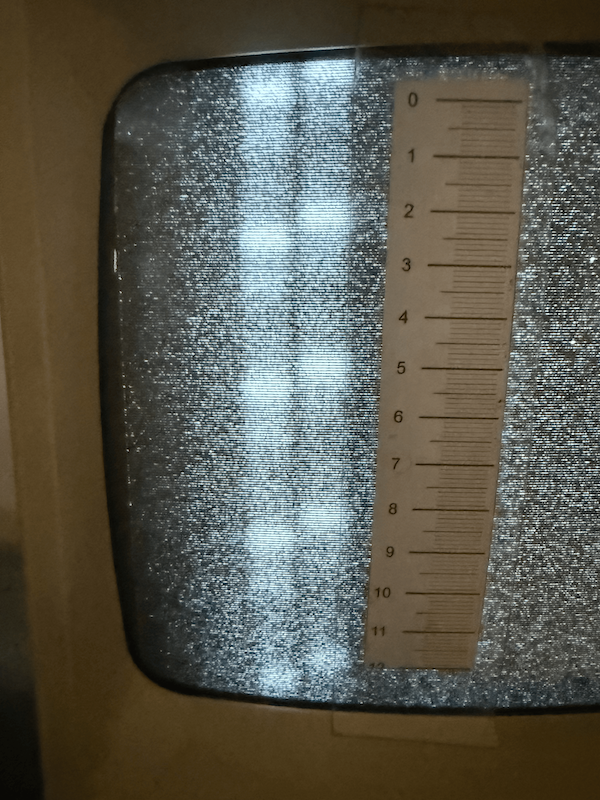
\includegraphics[width=0.3\textwidth]{pol1.png}
    \caption{Поляризация 1}
\end{figure}
\begin{figure}[H]
    \centering
    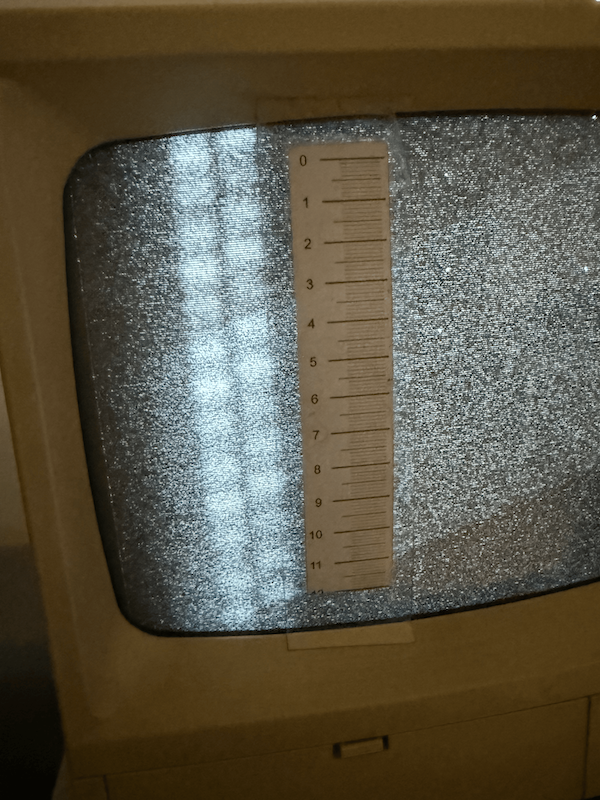
\includegraphics[width=0.3\textwidth]{pol2.png}
    \caption{Поляризация 2}
\end{figure}
Из этого можно сделать вывод, что:
\begin{itemize}
    \item \(\pi\)-компонента (несмещённая, \(\Delta M = 0\)) исчезает, когда ось поляризатора перпендикулярна направлению магнитного поля. Это означает, что она линейно поляризована \textbf{параллельно} вектору \(\vec{H}\).
    \item \(\sigma\)-компоненты (смещённые, \(\Delta M = \pm 1\)) исчезают, когда ось поляризатора параллельна \(\vec{H}\). Следовательно, они линейно поляризованы \textbf{перпендикулярно} направлению магнитного поля.
\end{itemize}
\section{Вывод}
Изучили характеристики интерферометра Фабри–Перо (ИФП) и исследовали эффект Зеемана на примере расщепления линии ртути
\end{document}
